\documentclass[xcolor={dvipsnames}]{beamer}
\usepackage{HECbeamer}
%  \usepackage{pgfpages}
%  \pgfpagesuselayout{4 on 1}[letterpaper,landscape, border shrink=5mm]
% \usepackage{listings}
% \usepackage{minted}
% \usemintedstyle{vs}
% \newcommand{\saskeyword}[1]{\textcolor{blue}{#1}}
% \newenvironment{sasminted}{\VerbatimEnvironment\begin{minted}[escapeinside=||,fontsize=\small,baselinestretch=1, samepage=true]{sas}}
%  {\end{minted}}

\uselanguage{French}
\languagepath{French}
\title[\color{white}{MATH60604 \S~2e - Coefficient de détermination}]{MATH60604 \\Modélisation statistique \\ \S~2e - Coefficient de détermination}
\author{}
\date{\today}
\institute{HEC Montréal\\
Département de sciences de la décision}
\date{} 

\begin{document}
\frame{\titlepage}


\begin{frame}
\frametitle{Coefficient de corrélation linéaire de Pearson}
\bi
\item Le coefficient de corrélation linéaire \alert{quantifie} la force de la relation \textbf{linéaire} entre deux variables $X$ et $Y$. 
\item Supposons que l’on étudie $n$ couples d’observations $(X_1, Y_1),\ldots,(X_n, Y_n)$, où $(X_i, Y_i)$ sont les valeurs $X$ et $Y$ pour le sujet $i$.
\item Le coefficient de corrélation de Pearson est
\begin{align*}
r=\frac{\widehat{\mathsf{Co}}(X,Y)}{\sqrt{\widehat{\mathsf{Va}}(X)\widehat{\mathsf{Va}}(Y)}} =\frac{\sum_{i=1}^n (X_i-\overline{X})(Y_i-\overline{Y})}{\sqrt{\sum_{i=1}^n(X_i-\overline{X})^2 \sum_{i=1}^n (Y_i-\overline{Y})^2}},\end{align*}
où $\overline{X}$ et $\overline{Y}$ sont les moyennes empiriques de $X$ et $Y$.
\ei
\end{frame}

\begin{frame}
\frametitle{Propriétés du coefficient de corrélation linéaire de Pearson}
\begin{tcolorbox}[colback=lightgray!30!white, colframe=lightgray!75!black, title=Propriétés du coefficient de corrélation linéaire de Pearson]
\bi
\item $-1 \leq r \leq 1$
\item $r=1$ ($r=-1$)  si et seulement si les $n$ points sont alignés sur une droite de pente positive (négative). En d'autres termes, il existe deux constantes $a$ et $b > 0$ $(b <0$) telles que $y_i=a+b x_i$ pour tout $i$.
\ei
\end{tcolorbox}
 \begin{center}
  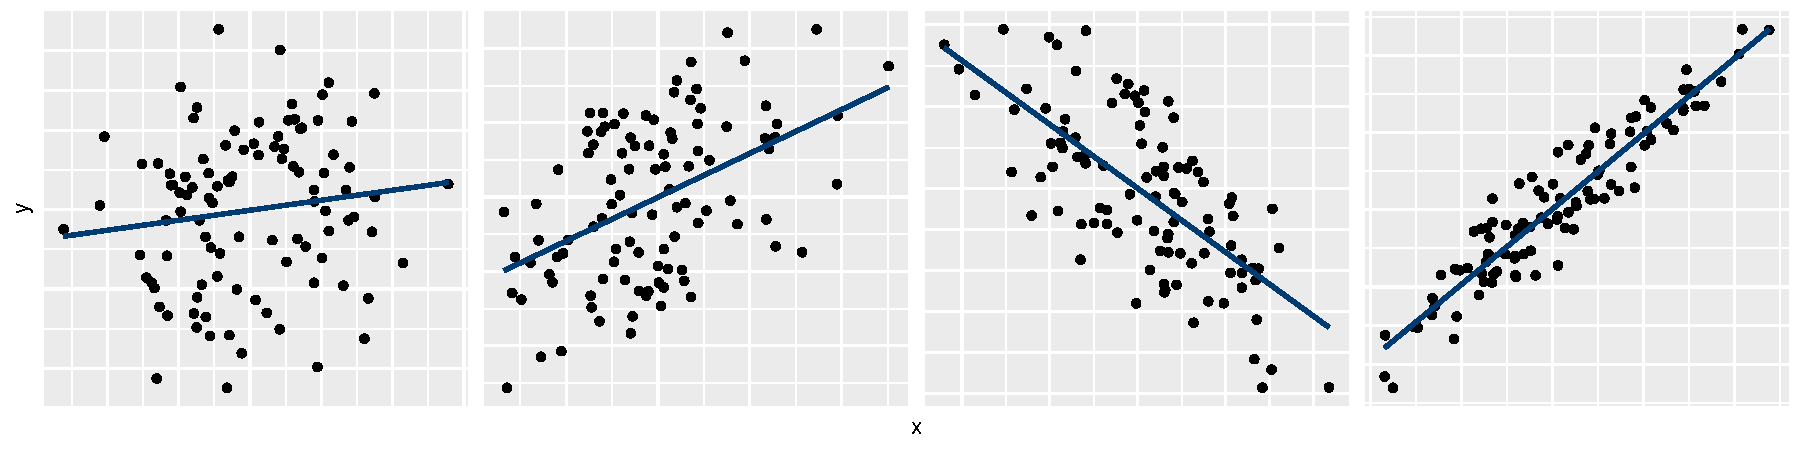
\includegraphics[width = \textwidth]{img/c2/03-linreg-correlation}
 \end{center}
{\footnotesize 
De gauche à droite, la corrélation linéaire est $0.1$, $0.5$, $-0.75$ et $0.95$.


}
 
\end{frame}


\begin{frame}[fragile]
\frametitle{Coefficient de corrélation linéaire de Pearson}
\bi
\item Si $r>0$ ($r<0$), les deux variables sont positivement (négativement) associées, ce qui veut dire que $Y$ augmente (diminue) en moyenne si $X$ augmente.
\item Plus $|r|$ est près de 1, moins les points sont éparpillés.
\item Deux variables indépendantes sont non corrélées (l'inverse est faux).
\item Une corrélation linéaire de zéro n'implique pas qu'il n'y a pas de relation entre les deux variables. Cela veut uniquement dire qu'il n'y a pas de dépendance \textbf{linéaire} entre les variables.

\ei

\begin{center}
 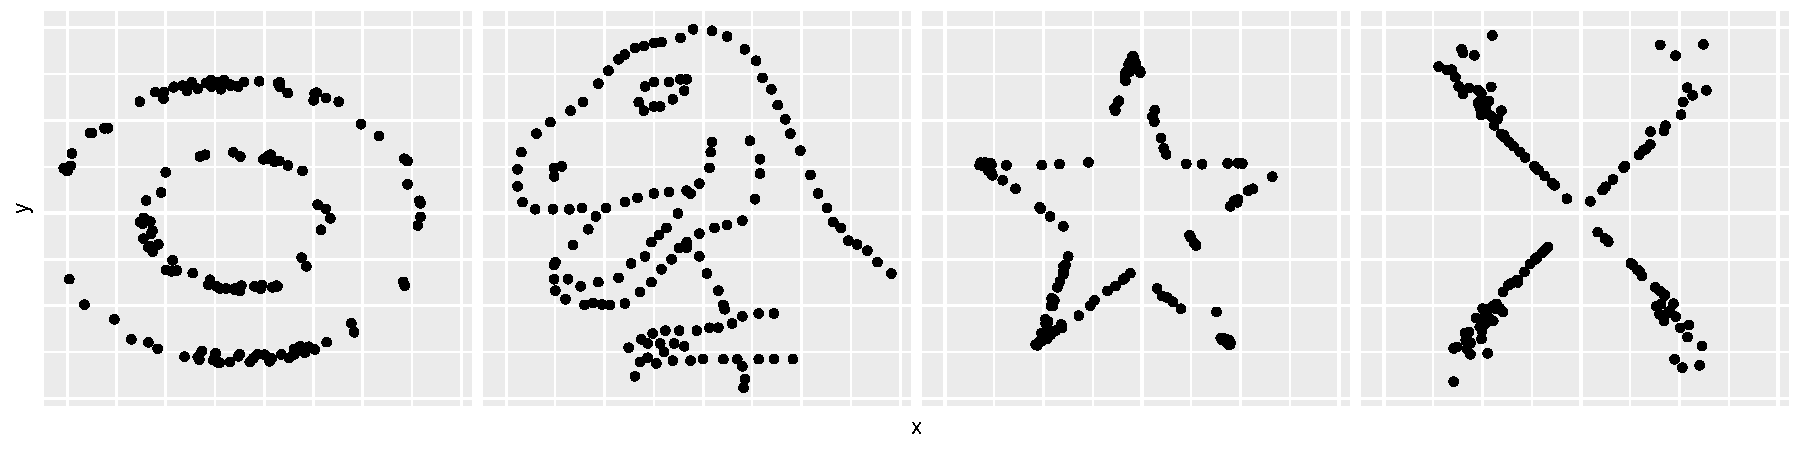
\includegraphics[width = 0.9\textwidth]{img/c2/03-linreg-datasaurus}
\end{center}
{\footnotesize
Les quatres jeux de données (cible,  Anscombosaurus, étoile, croix) ont une corrélation linéaire identique de $-0.06$, mais les variables ne sont clairement pas indépendantes.


}

\end{frame}

% \begin{frame}[fragile]
% \frametitle{  A picture is worth a thousand words}
% \begin{figure}
%  \centering
%  \includegraphics[width = 0.7\textwidth]{Figures/Anscombe_quartet.pdf}
% \end{figure}
% Anscombe's quartet: each dataset has $r=0.82$.
% \end{frame}

% \begin{frame}
% \frametitle{Pearson's linear correlation coefficient}
% \bi
% \item \alert{\textbf{Caution:}} It can be misleading to interpret the correlation coefficient without examining the scatterplot.  A few exemples in the next few pages will illustrate this.
% \item The following slides show scatterplots as well as the correlation coefficient in several situations where you'll have to use your own judgement.
% \item The last two exemples show the dangers of interpreting the correlation coefficient without having examined the scatterplot.
% \ei
% \end{frame}

\begin{frame}
\frametitle{Coefficient de détermination}
\bi
\item Une fois le modèle linéaire ajusté, il peut être utile d'avoir un résumé qui permet de quantifier la qualité de l'ajustement.
\item Le \alert{coefficient de détermination}, $R^2$, mesure la force de la relation linéaire entre $\hat{Y}$ et $Y$.  
\item Il représente la \alert{proportion de la variabilité} de $Y$ expliquée par les $\mathbf{X}$.
\item $R^2$ est le carré du coefficient de corrélation entre les valeurs ajustées et la réponse, $(\hat{Y}_1,Y_1),\ldots,(\hat{Y}_n,Y_n)$.
% \item Une définition formelle sera présentée dans les prochaines diapositives.
\ei
\end{frame}

\begin{frame}
\frametitle{Décomposition de la somme des carrés}
\bi
\item Supposons qu'aucune variable explicative n'est incluse dans le modèle (seulement l'ordonnée à l'origine). Dans ce cas, la valeur ajustée de $Y$ pour toutes les observations est la moyenne empirique et la somme du carré des observations centrées est
\begin{align*}
\mathsf{SS}_c=\sum_{i=1}^n (Y_i-\overline{Y})^2.                                      \end{align*}
\item Si le modèle inclut les régresseurs $\mathbf{X}$, la valeur ajustée de $Y_i$ est plutôt $\widehat{Y}_i=\widehat{\beta}_0+\sum_{j=1}^p\widehat{\beta}_1 \mathrm{X}_{ij}$ et la somme du carré des résidus du modèle est
\begin{align*}
\mathsf{SS}_e=\sum_{i=1}^n (Y_i-\widehat{Y}_i)^2.                                            \end{align*}
\item La valeur de $\mathsf{SS}_e$ ne croît jamais quand on ajoute des variables.
\ei
\end{frame}
% 
% \begin{frame}
% \frametitle{Sum of squares decomposition}
% \bi
% \item Define the sum of squared centered observations,
% \begin{align*}
% \mathsf{SS}_c=\sum_{i=1}^n (Y_i-\overline{Y})^2                                               \end{align*}
% 
% as the predicted value for each $Y_i$.
% \item When we include the $p$ regressors, the fitted value $Y_i$ is $\hat{Y}_i=\hat{\beta}_0+\hat{\beta}_1 \mathrm{X}_{i1}+\ldots+\hat{\beta}_p \mathrm{X}_{ip}$. Again, we define
% \begin{align*}
% \mathsf{SS}_e=\sum_{i=1}^n (Y_i-\hat{Y}_i)^2                                            \end{align*}
% as the sum of squared errors in the regression model including all the explanatory variables.

% \ei
% \end{frame}

\begin{frame}
\frametitle{Coefficient de détermination ($R^2$)}
\bi
\item $R^2$ mesure la proportion de la variance de $Y$ expliquée par les régresseurs $\mathrm{X}_1, \ldots, \mathrm{X}_p$,
\begin{align*}
R^2=\frac{\mathsf{SS}_c-\mathsf{SS}_e}{\mathsf{SS}_c}.                                                     \end{align*}
\item Quand il y a plus d'une variable explicative, la racine carrée de $R^2$ est appelé 
\alert{coefficient de corrélation multiple}. 
\item $R^2$ prend des valeurs entre $0$ et $1$

\ei
\end{frame}

% \begin{frame}
% \frametitle{Coefficient of determination}
% \bi
% \item Recall that
% \bi
% 
% \item $\mathsf{SS}_c$ is the error for the intercept-only model
% \item $\mathsf{SS}_e$ is the sum of squared residuals of the model with the covariates $\mathbf{X}$. 
% \ei
% % \item Consequently, $\mathsf{SS}_c-\mathsf{SS}_e$ is the reduction of the error associated with including $\mathbf{X}$ in the model, or rather, the proportion of the variation in $Y$ explained by $\mathbf{X}$.
% \item By dividing by $\mathsf{SS}_c$, we end up with
% \begin{align*}
% R^2=\frac{\mathsf{SS}_c-\mathsf{SS}_e}{\mathsf{SS}_c}                                                     \end{align*}
% This gives the proportion of the variability in $Y$ explained by $\mathbf{X}$.
% \ei
% \end{frame}
% 
% \begin{frame}
% \frametitle{Properties of the coefficient of determination}
% \begin{tcolorbox}[colback=lightgray!30!white, colframe=lightgray!75!black, title=Properties of the coefficient of determination]
% \bi
% \item $0 \leq R^2 \leq 1$
% \item $R^2$ is the squared correlation coefficient between the fitted values $\hat{\bs{Y}}$ and the response $\bs{Y}$, i.e. the correlation of $(Y_1,\widehat{Y}_1),\ldots,(Y_n,\widehat{Y}_n)$
% \ei
% \end{tcolorbox}
% \end{frame}
% 
% 

 \begin{frame}
\frametitle{Interprétation du coefficient de détermination}
\begin{center}
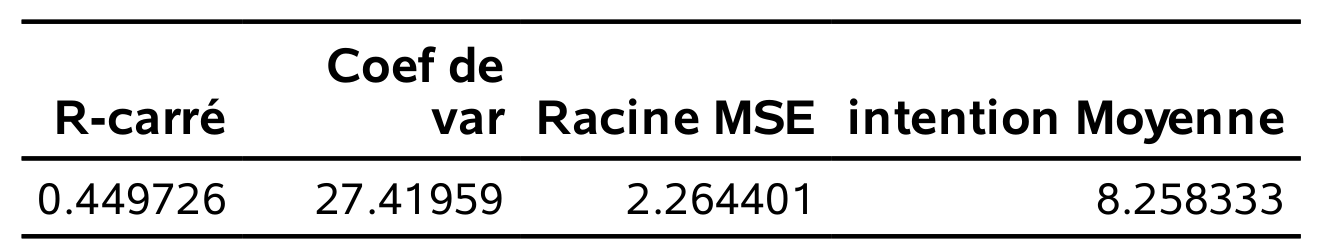
\includegraphics[width=0.6\linewidth]{img/c2/diapos3-e13}
\end{center}
\bi
\item Pour le modèle qui inclut toutes les variables explicatives,
$R^2=0.45$. Combinées, les variables expliquent $45\%$ de la variabilité d'\code{intention}.
\item Pour le modèle de régression linéaire simple avec \code{fixation} pour tout régresseur, 
$R^2 = 0.182$. Cela veut dire que la variable \code{fixation} explique  $18.2$\% de la variabilité d'\code{intention}.
\ei
\end{frame}

 \begin{frame}
 \frametitle{Avertissement au sujet de l'utilisation de $R^2$}
 \bi 
 \item 
 \textbf{Avertissement}: plus le nombre de régresseurs inclus est élevé, plus $R^2$ est grand (même si ces variables sont superflues à des fins d'inférence ou de prédictions).
  \item $R^2$ n'est donc pas un bon critère d'adéquation.
  \item Les logiciels rapportent parfois le coefficient de détermination ajusté, qui inclut une pénalité,  \[R^2_a=1-(1-R^{2})\frac{n-1}{n-p-1}. \]  
  Le coefficient perd en interprétabilité et peut être négatif.
  \ei 
  \end{frame}
  
  \end{document}
